\documentclass[]{article}
\usepackage[utf8]{inputenc}
\usepackage[left = 1.5cm, right = 1.5cm, top = 2cm, bottom = 2cm]{geometry}
\usepackage{cleveref}
\usepackage{graphicx}
\usepackage{float}
\title{RES}
\author{William Rooke\\12051342}
\date{\today}

\begin{document}

\maketitle

\section{Introduction}

\section{Pre-Work}
    \subsection{Explain the working principle of the PV emulator.}
        \begin{figure}[H]
        	\centering
        	\includegraphics*[width=0.75\textwidth]{PVDiagram}
        	\caption{Diagram of PV emulator and voltage control}
        \end{figure}
        It can be seen from the above diagram that
        \begin{equation}\label{eq:TotalCurrent}
            I_{pv} = I_{ph} - i_{Dpv} - i_p
        \end{equation}
        where the diode current $i_{Dpv}$ is given by
        \begin{equation}\label{eq:DiodeCurrent}
            i_{Dpv} = I_S (e^{\frac{V_D}{V_T}} - 1)
        \end{equation}
        and the thermal voltage of the diode $V_T$ is 
        \begin{equation}\label{eq:ThermalVoltage}
            V_T=\frac{K_B*T*A}{q}
        \end{equation}
        where A is the ideality factor of the solar cell, q is the charge of an electron, $K_B$ is the Boltzmann constant, T is the temperature in Kelvin and the voltage across the diode $V_D$ is
        \begin{equation}\label{eq:DiodeVoltage}
            V_D=V_{pv\_c}-I_{pv}*R_s
        \end{equation}
        The leakage current $I_p$ is given by
        \begin{equation}\label{eq:LeakageCurrent}
            i_p=\frac{V_{pv\_c}+I_{pv}*R_s}{R_{sh}}
        \end{equation}
        Combining \crefrange{eq:TotalCurrent}{eq:LeakageCurrent} gives the output current as
        \begin{equation}
            I_{pv}=I_{ph}-I_S(e^\frac{V_{pv\_c}-I_{pv}*R_s}{\frac{K_B*T*A}{q}}-1)-\frac{V_{pv\_c}+I_{pv}*R_s}{R_{sh}}
        \end{equation}
        As $R_{sh}$ does not affect the output voltage and is comparatively large compared to $R_s$, it can be ignored. Therefore, the power of the system is given by $P=I*V_{pv\_c}$ or
        \begin{equation}
            P=V_{pv\_c}*(I_{ph}-I_S(e^\frac{V_{pv\_c}-I_{pv}*R_s}{\frac{K_B*T*A}{q}}-1))
        \end{equation}
        The equation parameters $I_s$, $I_{ph}$ and $R_s$ can either found experimentally or from technical literature.
        \\
        The simulated PV emulator and the I-V and P-V curves from LTSpice are shown in \cref{fig:LTSpice,fig:IVCurve}
        \begin{figure}[H]
        	\centering
        	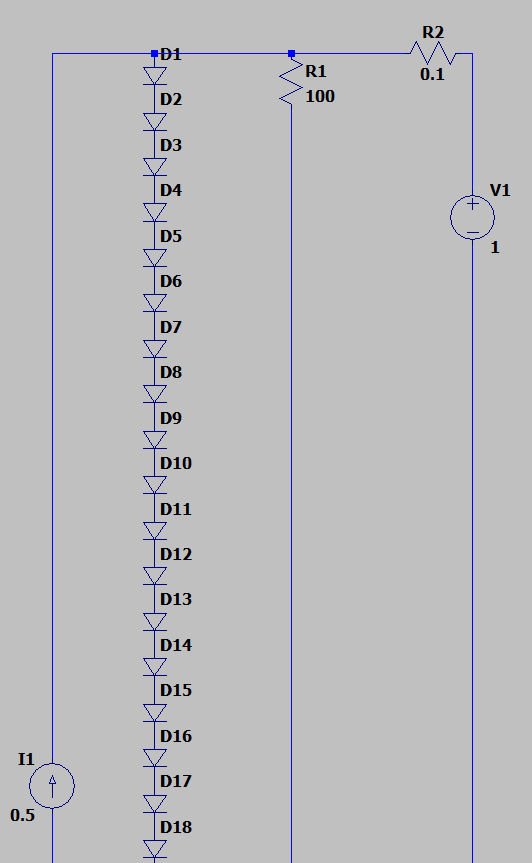
\includegraphics[width=0.5\textwidth]{LTSpice_cropped}
        	\caption{LTSpice circuit}
        	\label{fig:LTSpice}
        \end{figure}
       	\begin{figure}[H]
       		\centering
        	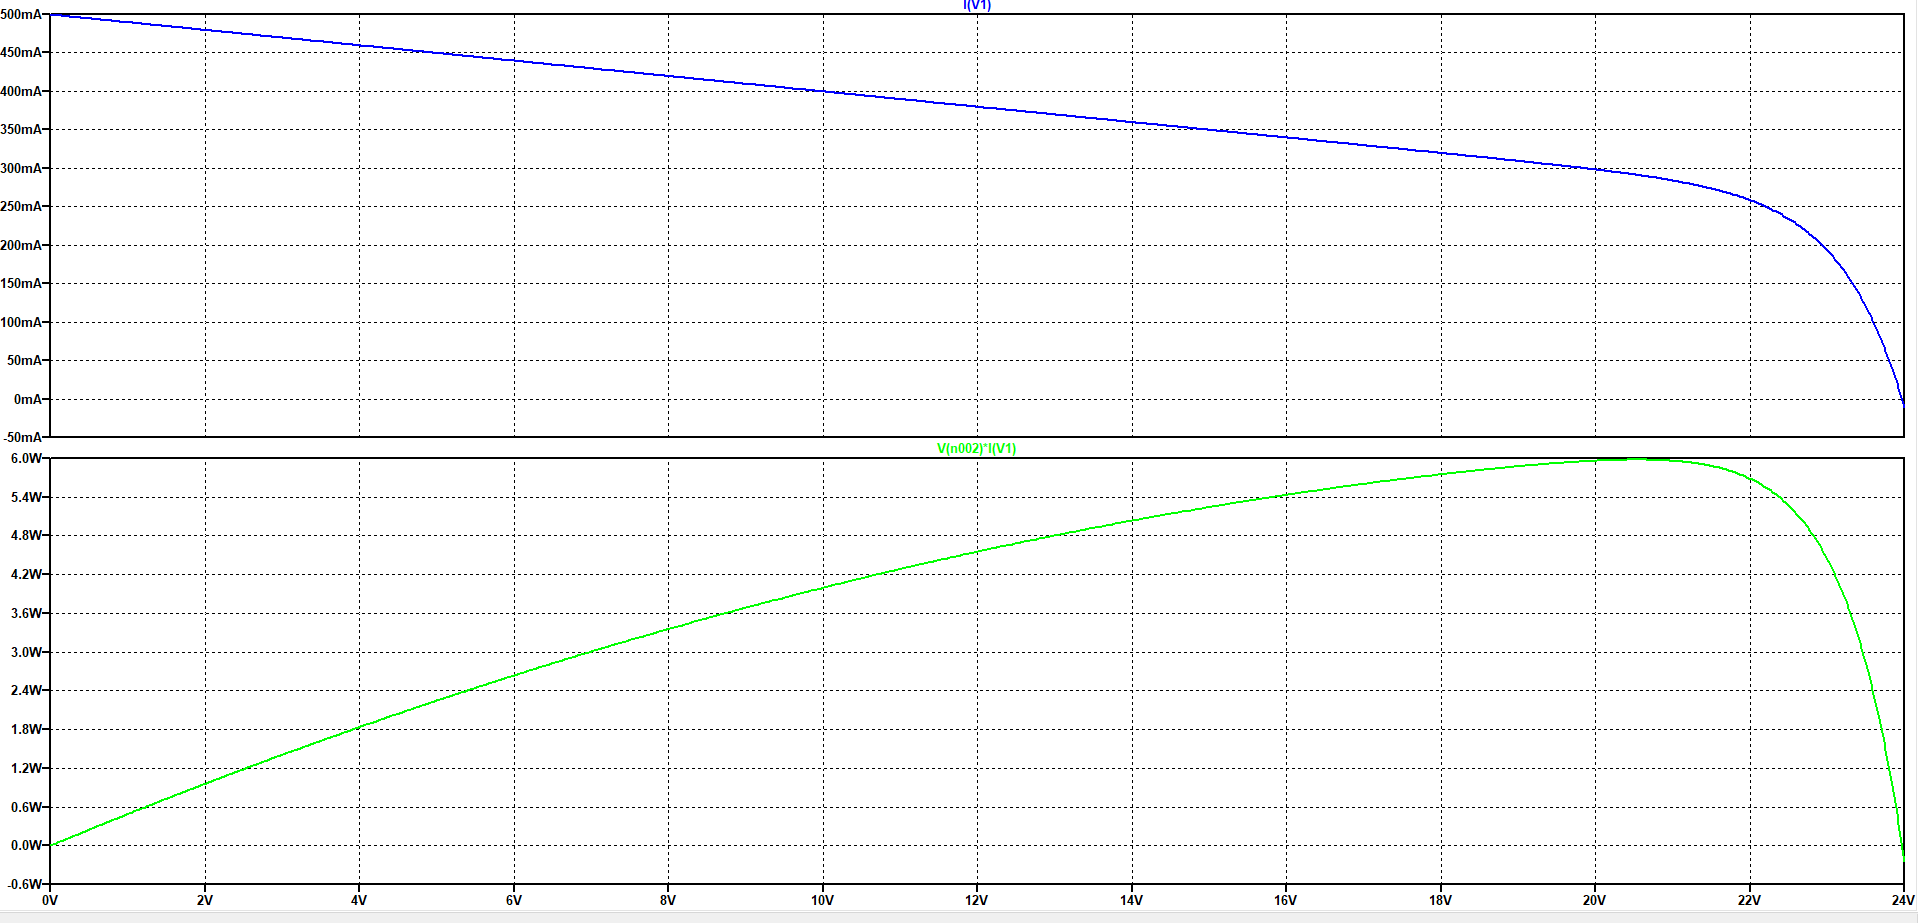
\includegraphics[width=\textwidth]{IVCurve}
        	\caption{I-V and P-V curves}
        	\label{fig:IVCurve}
        \end{figure}
    \subsection{Explain how the duty cycle should change to make the PV panel voltage constant and operate at the reference}
        If the PV panel voltage drops below the reference value, the duty cycle should be decreased in orer to bring the voltage back to the reference value. Similarly, if the PV voltage rises above the reference value, the duty cycle should be increased to ensure the PV voltage drops to the reference voltage.
\end{document}

